
\begin{frame}[t]{Walking without thinking}
\framesubtitle{Herdt and Wieber algorithm}

\begin{columns}[T]

\column[l]{0.5\textwidth}
\vspace*{2.0cm}
\begin{minipage}[t]{0.5\textwidth}
  \begin{center}
    \scalebox{0.7}{%!TEX root = ../../14-icra-RealTimeNMPC.tex

\tikzstyle{block} = [draw, fill=blue!20, rectangle,
    minimum height=2em, minimum width=5em, align=center]
\tikzstyle{sum} = [draw, fill=blue!20, circle, node distance=1cm]
\tikzstyle{input} = [coordinate]
\tikzstyle{output} = [coordinate]
\tikzstyle{pinstyle} = [pin edge={to-,thin,black}]

% The block diagram code is probably more verbose than necessary
\begin{tikzpicture}[auto, node distance=2cm,>=latex]
    % We start by placing the blocks
    \node [input]  at (-1, 0.0) (input)  {};
    \node [sum]    at ( 0.0, 0.0) (sumin)  {};
    \node [sum]    at ( 7.5, 0.0) (sumout) {};
    \node [output] at ( 8.0, 0.0) (output) {};

    % QP Controller Blocks
    \node [block] at (2,0) (oriqp) {
        QP Controller \\
        \small{Orientation}
    };
    \node [block] at (5.2,0) (posqp) {
        QP Controller \\
        \small{Position}
    };
    \node [block] at (3.5, -1.5) (system) {
    		System
    	};

    % PATHS
	% Forward chaine
    \draw [draw,->] (input) -- node {$
        \dot C_{k+1}^{ref}
    $} (sumin);
    \draw [->] (sumin) -- node {} (oriqp);
    \draw [->] (oriqp) -- node {$U_k^{\theta}$} (posqp);
    \draw [->] (posqp) -- node {$U_k^{x,y}$} (sumout);
    \draw [->] (sumout) -- node {} (output);

    % Feedback chaine
    \draw [->] (sumout) |- node {} (system);
    \draw [->] (system) -| node[above right] {$\hat{c}_k^{x,y,\theta}$, $\hat{f}_k^{x,y,\theta}$} (sumin);
\end{tikzpicture}


% The block diagram code is probably more verbose than necessary
%\begin{tikzpicture}[auto, node distance=2cm,>=latex']
%    % We start by placing the blocks
%    \node [input]  at (-0.5, 0.0) (input)  {};
%    \node [sum]    at ( 0.5, 0.0) (sumin)  {};
%    \node [sum]    at ( 6.5, 0.0) (sumout) {};
%    \node [output] at ( 7.5, 0.0) (output) {};
%
%    % QP Controller Blocks
%    \node [block] at (2.0,0) (oriqp) {
%        QP Controller\\
%        \small{Orientation}
%    };
%    \node [block] at (5.0,0) (posqp) {
%        QP Controller\\
%        \small{Position}
%    };
%    \node [block] at (5.0, -2.0) (dynamics) {Dynamics};
%    \node [block] at (2.0, -2.0) (system)   {System};
%
%    % PATHS
%    \draw [draw,->] (input) -- node {$
%        \dot C_{k+1}^{ref}
%    $} (sumin);
%    \draw [->] (oriqp) -- node {$U_k$} (posqp);
%    \draw [->] (posqp) -- node {$U_k$} (sumout);
%    \draw [->] (dynamics) --  (system);
%
%    \draw [->] (sumout) -- node {$ $} (output);
%    \draw [->] (sumin) -- node {} (oriqp);
%    \draw [->] (sumout) |- node[near start] {$y$}   (dynamics);
%    \draw [->] (system) -| node[near end]   {$val$} (sumin);
%\end{tikzpicture}
} \\
  \end{center}
\end{minipage}

\column{0.35\textwidth} 
\vspace*{1.5cm}
\begin{minipage}[t]{\textwidth}
  HRP-2 under actuation control compute the : 
  \begin{enumerate}
    \item {\color{black!20!red} CoM trajectory} w.r.t. a reference velocity
      ($\dot{c}_x,\;\dot{c}_y,\;\dot{c}_{\theta} $)
    \item {\color{black!20!red} feet positions and orientations} \footnotemark
  \end{enumerate}
\end{minipage}

\end{columns}
\footnotetext{\fullcite{herdt:iros:10}}
\end{frame}


\begin{frame}{Cost functions}
\framesubtitle{Cost functions (1/2)}
\tikzstyle{na} = [baseline=-.5ex]

\begin{itemize}
    \item tracking of a reference velocity
        \tikz[na] \node[coordinate] (n1) {};
\end{itemize}

% Below we mix an ordinary equation with TikZ nodes. Note that we have to
% adjust the baseline of the nodes to get proper alignment with the rest of
% the equation.
\begin{equation*}
  \min_{U_k^\theta} \quad \frac{\alpha}{2}
  \tikz[baseline]{
    \node[fill=green!20,anchor=base] (t1)
    {
      $ \lVert \dot{F}_{k+1}^\theta -
      \dot{C}_{k+1}^{\theta,ref} \rVert_2^2$
    };
  }
  \label{equ:Ori_QP_Problem}
\end{equation*}

\begin{center}
DoFs : $  
  U_k^{\theta} =
    \begin{bmatrix}
      \dddot F_k^{\theta,R} \\
      \dddot F_k^{\theta,L}
    \end{bmatrix} $
\end{center}

% Now it's time to draw some edges between the global nodes. Note that we
% have to apply the 'overlay' style.
\begin{tikzpicture}[overlay]
        \path[->,line width=0.5mm, green!50!black!70]<1-> (n1) edge [bend left] (t1);
\end{tikzpicture}

\end{frame}

\begin{frame}{Cost functions}
\tikzstyle{na} = [baseline=-.5ex]
\begin{itemize}
    \item tracking velocity
        \tikz[na] \node[coordinate] (n2) {};
    \item increase balance
        \tikz[na] \node[coordinate] (n3) {};
\end{itemize}
% Below we mix an ordinary equation with TikZ nodes. Note that we have to
% adjust the baseline of the nodes to get proper alignment with the rest of
% the equation.
\begin{align*}
  &\min_{U_{k}^{x,y}} \frac{\alpha}{2}
  \tikz[baseline]{
    \node[fill=green!20,anchor=base] (t2)
    {$ \lVert \dot C_{k+1}^{x} - \dot c_{ref}^{x} \rVert^2_2 $};
  }
  + \frac{\alpha}{2} 
  \tikz[baseline]{
    \node[fill=green!20,anchor=base] (t3)
    {$\lVert \dot C_{k+1}^{y} - \dot c_{ref}^{y} \rVert^2_2$};
  }
  + \frac{\gamma}{2}
  \tikz[baseline]{
    \node[fill=red!20,anchor=base] (t4)
    {$ \lVert F_{k+1}^{x} - ZMP_{k+1}^{x} \rVert^2_2$};
  }
  +\\
  & \frac{\gamma}{2} \tikz[baseline]{
    \node[fill=red!20,anchor=base] (t5)
    {$ \lVert F_{k+1}^{y} - ZMP_{k+1}^{y} \rVert^2_2$};
  }  
  + \frac{\delta}{2}
  \tikz[baseline]{
    \node[fill=blue!20,anchor=base] (t6)
    {$ \lVert \dddot C_{k+1}^{x} \rVert^2_2$};
  }  
  + \frac{\delta}{2}
  \tikz[baseline]{
    \node[fill=blue!20,anchor=base] (t7)
    {$ \lVert \dddot C_{k+1}^{y} \rVert^2_2$};
  }
\end{align*}
\begin{itemize}
    \item minimize the control
        \tikz[na] \node[coordinate] (n4) {};
\end{itemize}
\begin{center}
DoFs : $   
        U_k^{x,y} =
        \begin{bmatrix}
          \dddot C_{k}^x & F_{k}^x & \dddot C_{k}^y & F_{k}^y
        \end{bmatrix}^T
         $
\end{center}

% Now it's time to draw some edges between the global nodes. Note that we
% have to apply the 'overlay' style.
\begin{tikzpicture}[overlay]
        \path[->,line width=0.5mm, green!50!black!70]<2-> (n2) edge [bend left] (t2);
        \path[->,line width=0.5mm, green!50!black!70]<2-> (n2) edge [bend left] (t3);
        \path[->,line width=0.5mm, red!100!black!80]<3-> (n3) edge [bend left] (t4);
        \path[->,line width=0.5mm, red!100!black!80]<3-> (n3) edge [bend left] (t5);
        \path[->,line width=0.5mm, blue!50!black!70]<4-> (n4) edge [bend right] (t6);
        \path[->,line width=0.5mm, blue!50!black!70]<4-> (n4) edge [bend right] (t7);
\end{tikzpicture}


\end{frame}


%%
%\begin{frame}{Cost functions}
%%\framesubtitle{Constraints}
%\begin{columns}
%    \column{0.1\textwidth}
%    \begin{cadre}
%    \end{cadre}
%    \column{0.8\textwidth}    
%    \begin{cadre}
%        \begin{flalign}
%            \min_{U_k^\theta} \quad \frac{\alpha}{2} \lVert \dot{F}_{k+1}^\theta -
%                \dot{C}_{k+1}^{\theta,ref} \rVert_2^2 & &
%            \label{equ:Ori_QP_Problem}
%        \end{flalign} 
%        DoFs : $ 
%        U_k^{\theta} =
%            \begin{bmatrix}
%                \dddot F_k^{\theta,R} \\
%                \dddot F_k^{\theta,L}
%            \end{bmatrix}
%        $\\
%        \begin{flalign}
%            \min_{U_{k}^{x,y}} &
%            \frac{\alpha}{2} \lVert \dot C_{k+1}^{x} - \dot c_{ref}^{x} \rVert^2_2
%            + \nonumber
%            \frac{\alpha}{2} \lVert \dot C_{k+1}^{y} - \dot c_{ref}^{y} \rVert^2_2\\
%            + &
%            \frac{\gamma}{2} \lVert F_{k+1}^{x} - ZMP_{k+1}^{x} \rVert^2_2
%            + \nonumber
%            \frac{\gamma}{2} \lVert F_{k+1}^{y} - ZMP_{k+1}^{y} \rVert^2_2 \\
%            + &
%            \frac{\delta}{2} \lVert \dddot C_{k+1}^{x} \rVert^2_2
%            +
%            \frac{\delta}{2} \lVert \dddot C_{k+1}^{y} \rVert^2_2
%            \label{equ:Pos_QP_Problem} & &
%        \end{flalign} 
%
%        with
%        DoFs : $ 
%        U_k^{x,y} =
%        \begin{bmatrix}
%          \dddot C_{k}^x & F_{k}^x & \dddot C_{k}^y & F_{k}^y
%        \end{bmatrix}^T
%        $
%    \end{cadre}
%    \column{0.1\textwidth}
%    \begin{cadre}
%    \end{cadre}
%\end{columns}
%\end{frame}



\begin{frame}{Constraints}
%\framesubtitle{}
\begin{columns}
    \column{0.5\textwidth}
    \begin{cadre}
      \begin{center}
        \scalebox{0.7}{%!TEX root = ../../NMPC_WPG.tex

\newcommand{\tetazero}{20.55}
\newcommand{\Fkxzero}{-20}
\newcommand{\Fkyzero}{20}

\newcommand{\tetaone}{-20}
\newcommand{\Fkxone}{5}
\newcommand{\Fkyone}{0}

\newcommand{\tetatwo}{20}
\newcommand{\Fkxtwo}{25}
\newcommand{\Fkytwo}{20}

%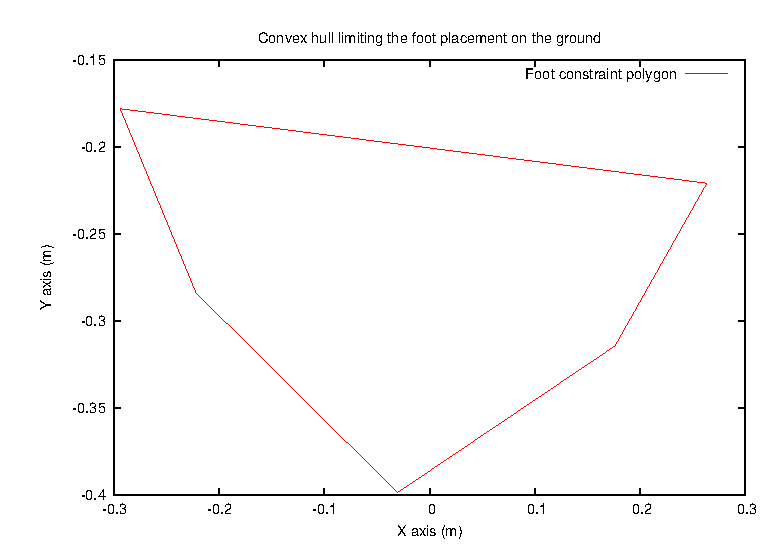
\includegraphics[width=15cm]{./figures/walking-without-thinking/ConvexHull}
\begin{tikzpicture}[scale=0.075]
\draw [dashed][->](-50,0) -- (50,0) node [below left, black]{$\overrightarrow{x}$}; %x-axis
\draw [dashed][->](0,-50) -- (0,50) node [below left, black]{$\overrightarrow{y}$}; %y-axis
 %right support, left foot landing convexhull
\draw (-28,-20)--(-20,-30)--(0,-40)--(20,-30)--(28,-20)--(-28,-20) node [below left, black]{$A^r_0$,$B^r_0$} ;
 %left support, right foot landing convexhull
\draw (-28,20)--(-20,30)--(0,40)--(20,30)--(28,20)--(-28,20) node at (-10,30)[black]{$A^l_0$,$B^l_0$} ;
 %support foot
\draw (-10,-5)--(10,-5)--(10,5)--(-10,5)--(-10,-5) node [below left, black]{Support Foot} ;

% rotated support foot
\draw [dotted][cm={cos(\tetazero) ,sin(\tetazero) ,-sin(\tetazero) ,cos(\tetazero) ,(0.0 cm,0.0 cm)}]
(-10,-5)--(10,-5)--(10,5)--(-10,5)--(-10,-5) ;
% rotated axis
\draw [dotted][-][cm={cos(\tetazero) ,sin(\tetazero) ,-sin(\tetazero) ,cos(\tetazero) ,(0.0 cm,0.0 cm)}]
(0,0) -- (30,0) node [below left, black]{};
% angle
\draw (0,0) -- (18.727324381,7.02049297) arc (\tetazero:0:20) -- (0.0,0.0) node at (21,5) {$\theta$} ;
% rotated left support, right foot landing convexhull
\draw [dotted][-][cm={cos(\tetazero) ,sin(\tetazero) ,-sin(\tetazero) ,cos(\tetazero) ,(0.0 cm,0.0 cm)}]
(-28,20)--(-20,30)--(0,40)--(20,30)--(28,20)--(-28,20) ;
% rotated right support, left foot landing convexhull
\draw [dotted][-][cm={cos(\tetazero) ,sin(\tetazero) ,-sin(\tetazero) ,cos(\tetazero) ,(0.0 cm,0.0 cm)}]
(-28,-20)--(-20,-30)--(0,-40)--(20,-30)--(28,-20)--(-28,-20);

\draw [thick][dashed][->](0,0) -- (-28,20) node [black] at (-33.0,20.0){${\bf p}_1^l$}; %y-axis
\draw [thick][dashed][->](0,0) -- (-20,30) node [black] at (-25.0,32.0){${\bf p}_2^l$}; %y-axis
\draw [thick][dashed][->](0,0) -- (0.0,40) node [black] at (5.0,42.0){${\bf p}_3^l$}; %y-axis
\draw [thick][dashed][->](0,0) -- (20,30) node [right, black]{${\bf p}_4^l$}; %y-axis
\draw [thick][dashed][->](0,0) -- (28,20) node [right, black]{${\bf p}_5^l$}; %y-axis

\end{tikzpicture}
}
      \end{center}               
    \end{cadre}
    \column{0.6\textwidth}
    \begin{cadre}
        \begin{enumerate}
            \item ZMP constraint :
                \begin{itemize}
                  \item $ {\bf d} _i R(f_k^\theta) \left( {\bf Z}_k -
                      {\bf f}_k \right) \leq {\bf d} _i {\bf p} _i. $*
                \end{itemize}
             \item Foot position constraint :
                \begin{itemize}
                  \item ${\bf d}_i R(f_k^\theta) ({\bf f}_{k+1} - {\bf f}_k )
                     \leq {\bf d}_i {\bf p}_i $*
                \end{itemize}
  
              \item[*] with $ {\bf d}\,_i :=
                  \begin{bmatrix}
                      p_{i}^y-p_{i+1}^y & p_{i+1}^{x}-p_{i}^{x}
                  \end{bmatrix} $
                  $ \forall i = 1,...,n_\textup{edges} $\\
                      $ \text{with} \,p_{n_\textup{edges}+1}\,:=p_1 $
            \end{enumerate}
        \end{cadre}
    \end{columns}
\end{frame}

\begin{frame}[t]{Walking without thinking}
\framesubtitle{Combined QP = SQP}

\begin{columns}[T]

\column[l]{0.5\textwidth}
\vspace*{2.5cm}
\begin{minipage}[t]{0.5\textwidth}
  \begin{center}
    \scalebox{0.8}{%!TEX root = ../../14-icra-RealTimeNMPC.tex

\tikzstyle{block} = [draw, fill=blue!20, rectangle,
    minimum height=2em, minimum width=5em, align=center]
\tikzstyle{sum} = [draw, fill=blue, circle, node distance=1cm]
\tikzstyle{input} = [coordinate]
\tikzstyle{output} = [coordinate]
\tikzstyle{pinstyle} = [pin edge={to-,thin,black}]

% The block diagram code is probably more verbose than necessary
\begin{tikzpicture}[auto, node distance=2cm,>=latex]
\normalsize
    % We start by placing the blocks
    \node [input]  at (-2, 0.0) (input)  {};
    \node [sum]    at ( -0.5, 0.0) (sumin)  {};
    \node [sum]    at ( 7.5, 0.0) (sumout) {};
    \node [output] at ( 8.5, 0.0) (output) {};

    % SQP Controller Block
    \node [block] at (3.5,0) (controller) {
        \normalsize real time SQP Controller \\
        \normalsize Orientation $+$ Position
    };
    % System Block
    \node [block] at (3.5, -2) (system) {
            \normalsize Generalized Inverse Kinematics\\
             \normalsize Robot
        };
    
    % PATHS
    \draw [draw,->] (input) -- node {$
        \mathbf{v}^{\mathrm{ref}}
    $} (sumin);
    \draw [->] (controller) -- node[name=u, align=center] {
    $\begin{matrix}
        \hat{c}_{k+1}^{x,y,\theta}\\
        \hat{f}_{k+1}^{x,y,\theta}
    \end{matrix}$
    } (sumout);
    \draw [draw,->] (sumout) -- node {$
    $} (output);
    \draw [->] (sumin) -- node {} (controller);
    \draw [->] (sumout) |- node[near start] {}   (system);
    \draw [- ] (sumout) |- node {} (-0.5, -1.0);
    \draw [->] (-0.5, -1.0) -- node {} (sumin);

\end{tikzpicture}
} \\
  \end{center}
\end{minipage}

\column{0.35\textwidth} 
\vspace*{1.5cm}
\begin{minipage}[t]{\textwidth}
  HRP-2 under actuation control compute : 
    \begin{enumerate}
    \item the CoM trajectory w.r.t. a
        reference velocity ($\dot{c}_x,\;\dot{c}_y,\;\dot{c}_{\theta} $)
    \item the feet positions and orientations
    \end{enumerate}
  Nice feature embedded (obstacle avoidance, ...)\\
  Cost $2\times$ in computation times
\end{minipage}
\end{columns}
\end{frame}

\begin{frame}{Experiment on HRP2}
  \begin{center}
    \movie[autostart,loop]{
    
\includegraphics[width=0.85\linewidth, keepaspectratio]
      {16-raletter-NMPC-v19.png}    
    }  
    {videos/16-raletter-NMPC-v19.mp4}
  \end{center}
\end{frame}

\begin{frame}
  \frametitle{Reactive walking pattern generation \only<4>{with obstacles}} 
  \begin{columns}
    \begin{column}{0.6\linewidth}
      \vskip 1cm
      Optimization problem solved:
      \only<1-3>{
        \begin{equation*}
          \begin{aligned}
            \min_{{\bf U}_k} 
            \sum_{i=0}^{j=4} w_i J_i({\bf U}_{k}) & \\
                {\bf X}_{k+1} = {\bf A}{\bf X}_{k} + {\bf C} {\bf U}_k & \\
                \underline{\bf P} < {\bf P} {\bf U}_k  < \overline{\bf P}& \\
          \end{aligned}
        \end{equation*}
        with ${\bf U}_k=\begin{pmatrix} \dddot{\bf X}_k \; {\bf X}_k^\mathit{f}\; \dddot{\bf Y}_k \;{\bf Y}_k^\mathit{f}  \end{pmatrix}^T$ \\        
      }
      \only<4>{
        \begin{equation*}
          \begin{aligned}
            \min_{{\bf U}_k} 
            \sum_{i=0}^{j=4} w_i J_i({\bf U}_{k}) & \\
                {\bf X}_{k+1} = {\bf A}{\bf X}_{k} + {\bf C} {\bf U}_k & \\
                \underline{\bf P} < {\bf P}{\color{red}{({\bf U}_k)}} {\bf U}_k  < \overline{\bf P}& \\
          \end{aligned}
        \end{equation*}
      with ${\bf U}_k=\begin{pmatrix} \dddot{\bf X}_k \; {\bf X}_k^\mathit{f}\; \dddot{\bf Y}_k \;{\bf Y}_k^\mathit{f} \;\color{red}{{\bf \Theta}_k^\mathit{f}}\end{pmatrix}^T$ \\
      }
     \end{column}
     \begin{column}{0.45\linewidth}
       \only<1-3>{
         \begin{tikzpicture}[remember picture, overlay]
           \node[minimum width=5cm] at ([xshift=3.0cm,yshift=-0.25cm]current page.center)
                {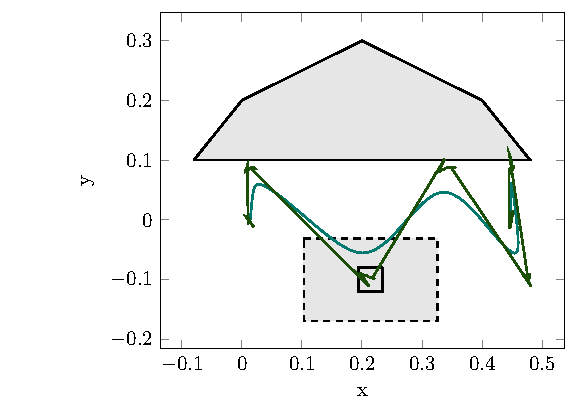
\includegraphics[width=\linewidth]{./images/tikz/convexHulls2}};
           \node[font=\small,text ragged] at ([xshift=0.0cm,yshift=+3.0cm]current page.center)
                     {\textcolor{blue}{[M. Naveau, RA-L 2016 accepted]}};
         \end{tikzpicture}
       }
       \only<4>{
          \begin{tikzpicture}[remember picture, overlay]
            \node[minimum width=5cm] at ([xshift=3.0cm,yshift=-0.25cm]current page.center)
                 {\href{run://home/ostasse/Videos/Koroibot/Koroibot-HRP2-NMPC-v18.mp4}
                   {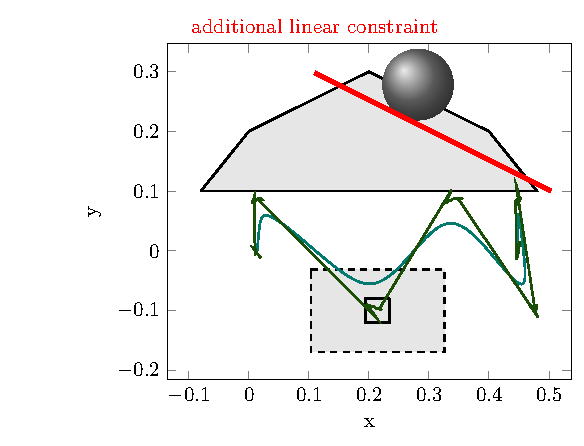
\includegraphics[width=\linewidth]{./images/tikz/convexHullsplusObstacles2}}};
            \node[font=\small,text ragged] at ([xshift=0.0cm,yshift=+3.0cm]current page.center)
               {\textcolor{blue}{[M. Naveau, RA-L 2016 accepted]}};
          \end{tikzpicture}
       }

     \end{column}
   \end{columns}
  \vskip 0.4cm
    \only<1>{
       $J_1({\bf U}_{k})$ is the linear velocity tracking 
         {\small
           \begin{equation*}
               J_1({\bf U}_k) = \lVert \dot {\bf X}_{k} - {\bf X}_{k}^{ref} \rVert^2_2
               +  \lVert \dot {\bf Y}_{k} - {\bf Y}_{k}^{ref} \rVert^2_2 
           \end{equation*}}
    }
    \only<2>{$J_2({\bf U}_{k})$ is the control norm
      {\small
        \begin{equation*}
          J_2({\bf U}_k) = \lVert \dddot {\bf X}_{k} \rVert^2_2
          + \lVert \dddot {\bf Y}_{k} \rVert^2_2
        \end{equation*}
      }
    }
    \only<3>{$J_3({\bf U}_{k})$ is distance of the CoP to the most stable trajectory
      {\small
        \begin{equation*}
          J_3({\bf U}_k) = \lVert {\bf X}_{k}^{f} - CoP_{k+1}^{x} \rVert^2_2 +
          \lVert {\bf Y}_{k+1}^{f} - CoP_{k+1}^{y} \rVert^2_2 
        \end{equation*}
      }
    }
    \only<4>{$J_4({\bf U}_{k})$ is the angular velocity tracking
      {\small
          \begin{equation*}
            J_4({\bf U}_k) = \lVert {\bf \Theta}_{k} - \int {\bf \Theta}_{k}^{ref} dt \; \rVert_2^2 
      \end{equation*}}
    }
\end{frame}